\documentclass[12pt]{article}
\title{ECE 11L Lab Report 1}

\author{Lawrence Liu}
\usepackage{graphicx}
\usepackage{amsmath}
\usepackage{subcaption}
\usepackage{array}

\begin{document}
\begin{titlepage}
   \begin{center}
       \vspace*{1cm}

       \textbf{EE 11L: Circuits Laboratory I}

       \vspace{2cm}

       \textbf{Experiment \#2}\\
       \textbf{Simple Resistive Networks}

            
       \vspace{4cm}
     
            
       Name: Lawrence Liu\\
		UID: 405749034\\
		Due Date: Nov. 11, 2100
            
   \end{center}
\end{titlepage}
\section*{Objectives}
To understand how to apply Thevenin and Norton equivalence theorems. To experimentally verify and measure the principle of superposition. To understand the operation of the Wheatstone bridge, and to apply to constructing circuits with sensors. 
\section*{Theory}
\textbf{Superposition}: For a linear circuit, the voltage at any node or current at any 
branch can is the algebraic sum of the caused by each source acting alone.\\\\
\textbf{Norton and Thevenin Equivalent Circuits}: A source Circuit can be converted to its Norton and Thevenin Equivalent Circuits.\\
\\
The Thevenin equivalent circuit would consist of a voltage source $V_{th}$ in series with a resistor $R_{th}$. $V_{th}$ is just the voltage across the terminals when open circuited. $R_{th}$ can be found by setting all the independent sources to $0$, ie replacing all voltage sources with shorts and replacing all current sources with an open circuit.
\\
The Norton equivalent circuit consists of a current source $I_{no}$ in parallel with a resistor $R_{no}$. $R_{no}=R_{th}$ and we can find $I_{no}$ by shorting the terminals and measuring the resistance that flows across.
\pagebreak
\section*{Experiment Setup: Lab 1}
\begin{figure}[h]
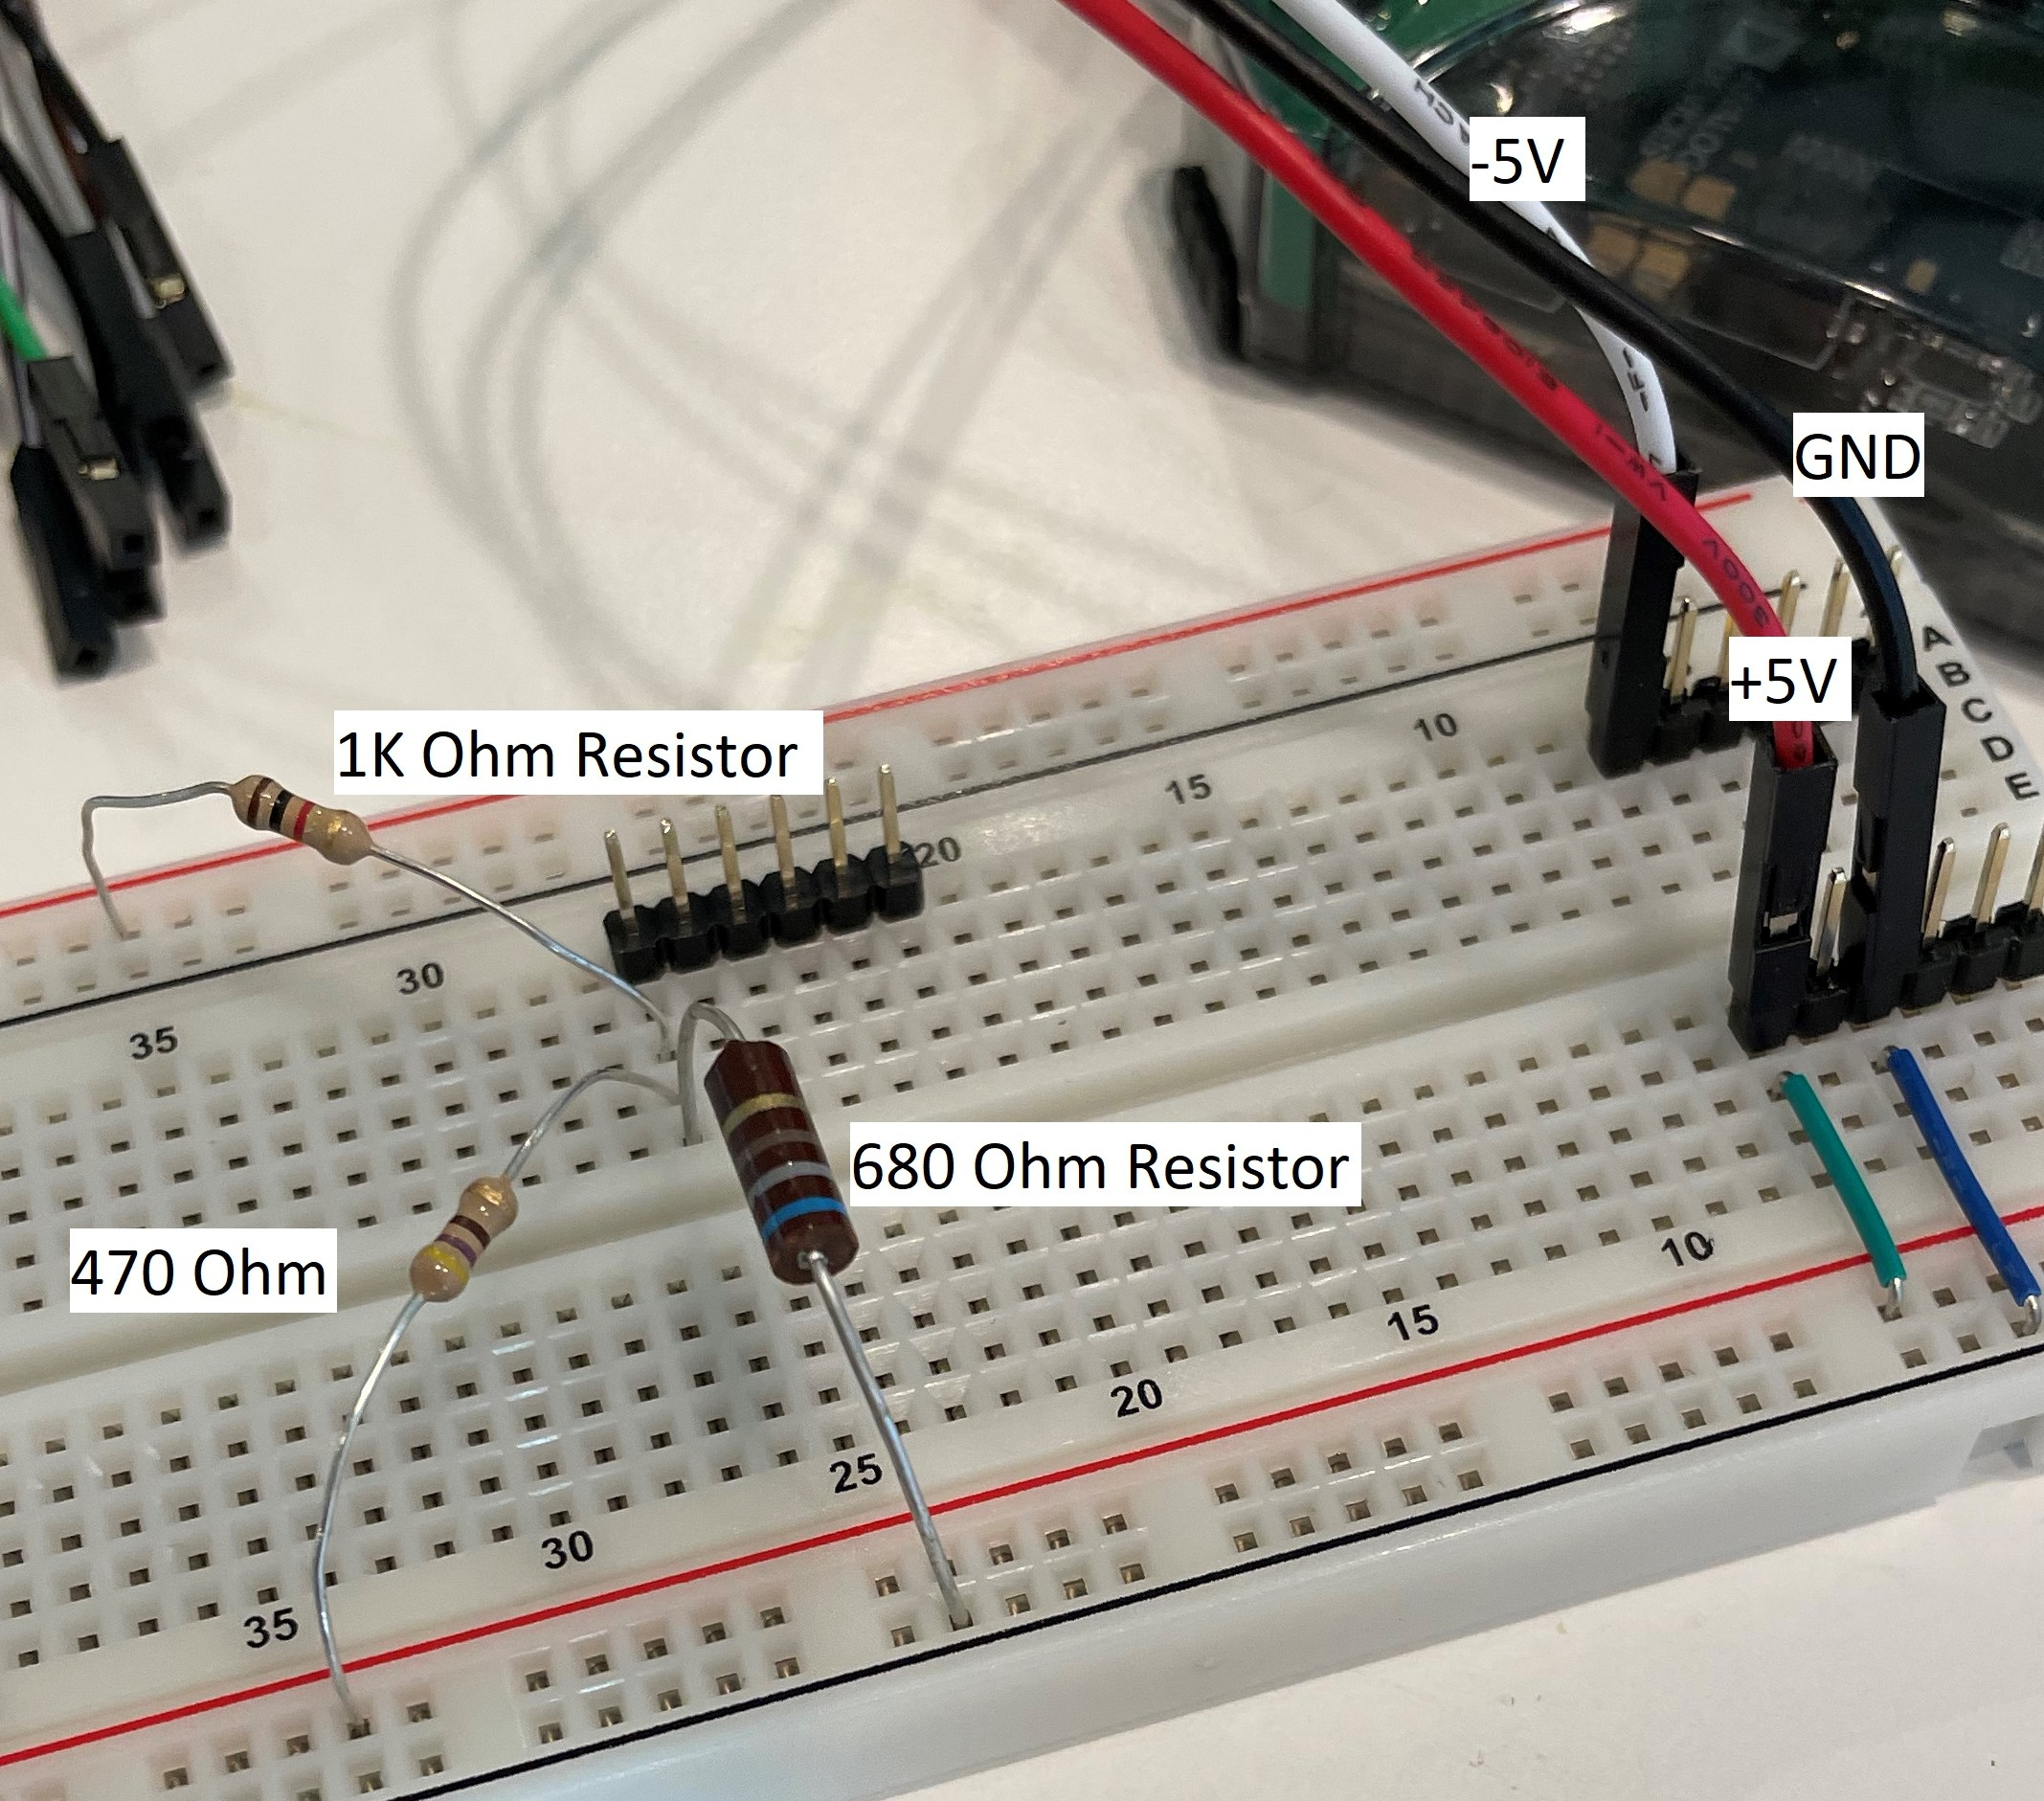
\includegraphics[width=8cm]{Lab 1}
\centering
\caption{Lab 1 Setup}
\end{figure}
\section*{Measurements: Lab 1}
\begin{center}
\begin{tabular}{||c|c|c ||}
\hline
Sources & Voltage (V) & Current (A)\\
\hline
\hline
$+5V$ only &2.38V &3.5mA\\
\hline
$-5V$ only &-1.153V &-1.7mA\\
\hline
Sum &1.227V &1.804mA\\
\hline
Both on & 1.253V&1.8mA\\
\hline
\end{tabular}
\end{center}
The theoretical calculations for the voltage across $R_3$ from the +5V source only is 2.3135V. The theoretical calculations for the voltage across $R_3$ from the -5V source only is -1.087V. The theoretical calculations for the voltage across $R_3$ from both sources is 1.226V.
\pagebreak
\section*{Discussion: Lab 1}
The difference between the theoretical and measured voltage for the voltage across $R_3$ from the +5V source is $2.8\%$. The difference between the theoretical and measured voltage for the voltage across $R_3$ from the -5V source is $5.69\%$.  The difference between the theoretical and measured voltage for the voltage across $R_3$ with both sources on is $2.1\%$.
\pagebreak
\section*{Experiment Setup: Lab 2}
\begin{figure}[h]
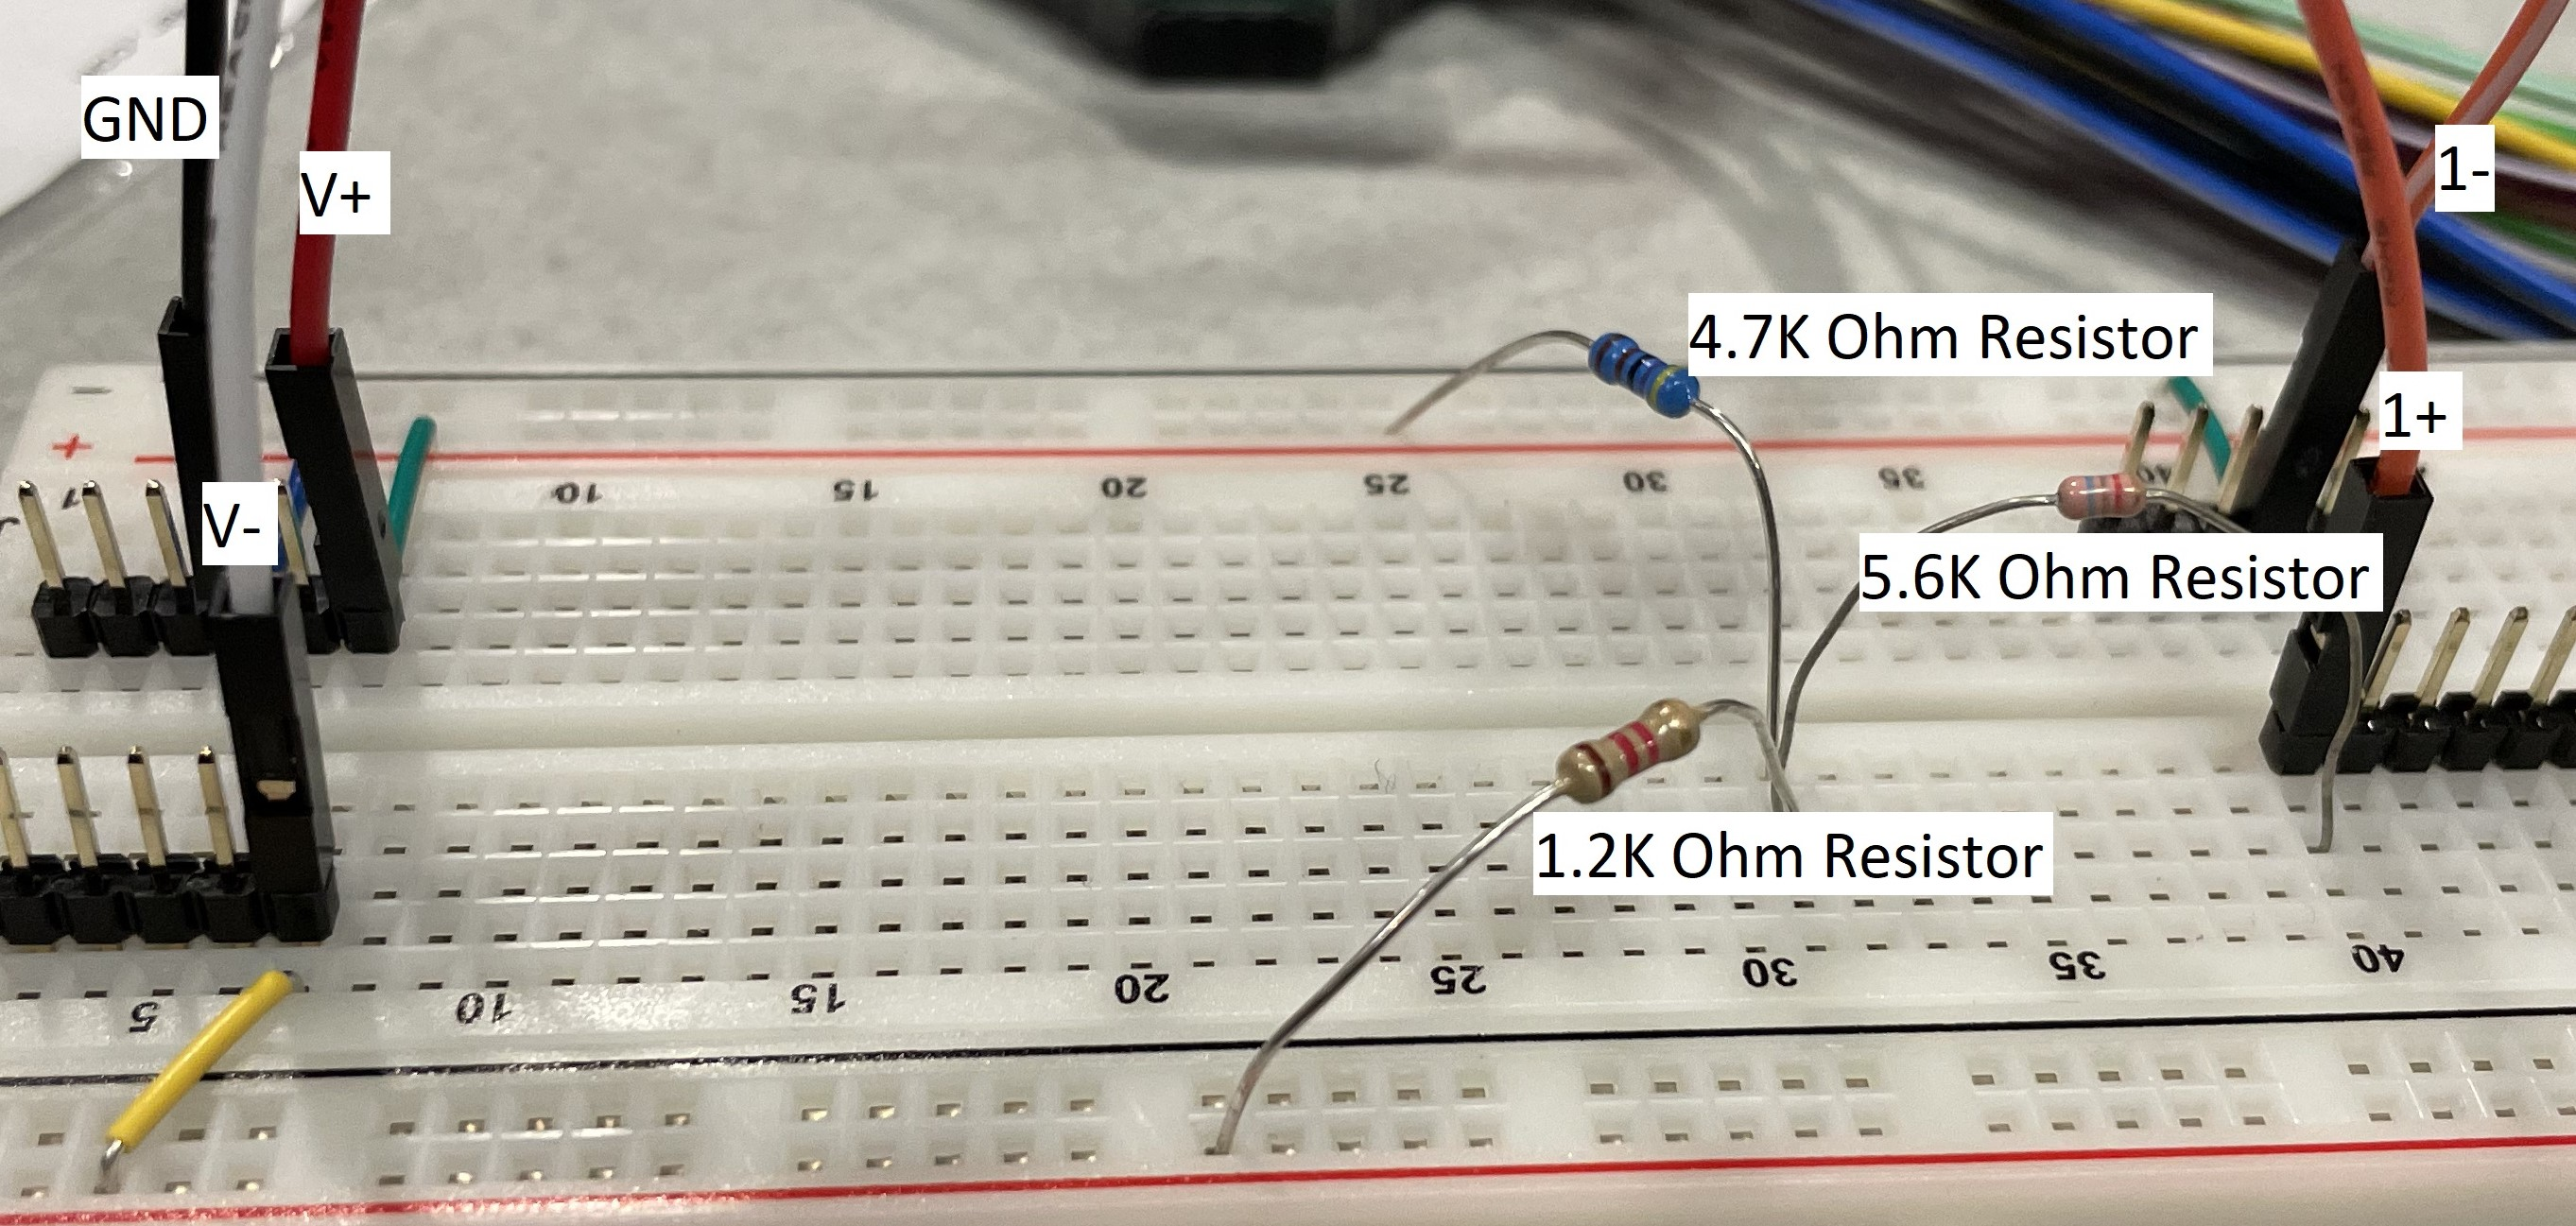
\includegraphics[width=8cm]{Lab2 Circuit}
\centering
\caption{Lab 2 Open Source Circuit}
\end{figure}
\begin{figure}[h]
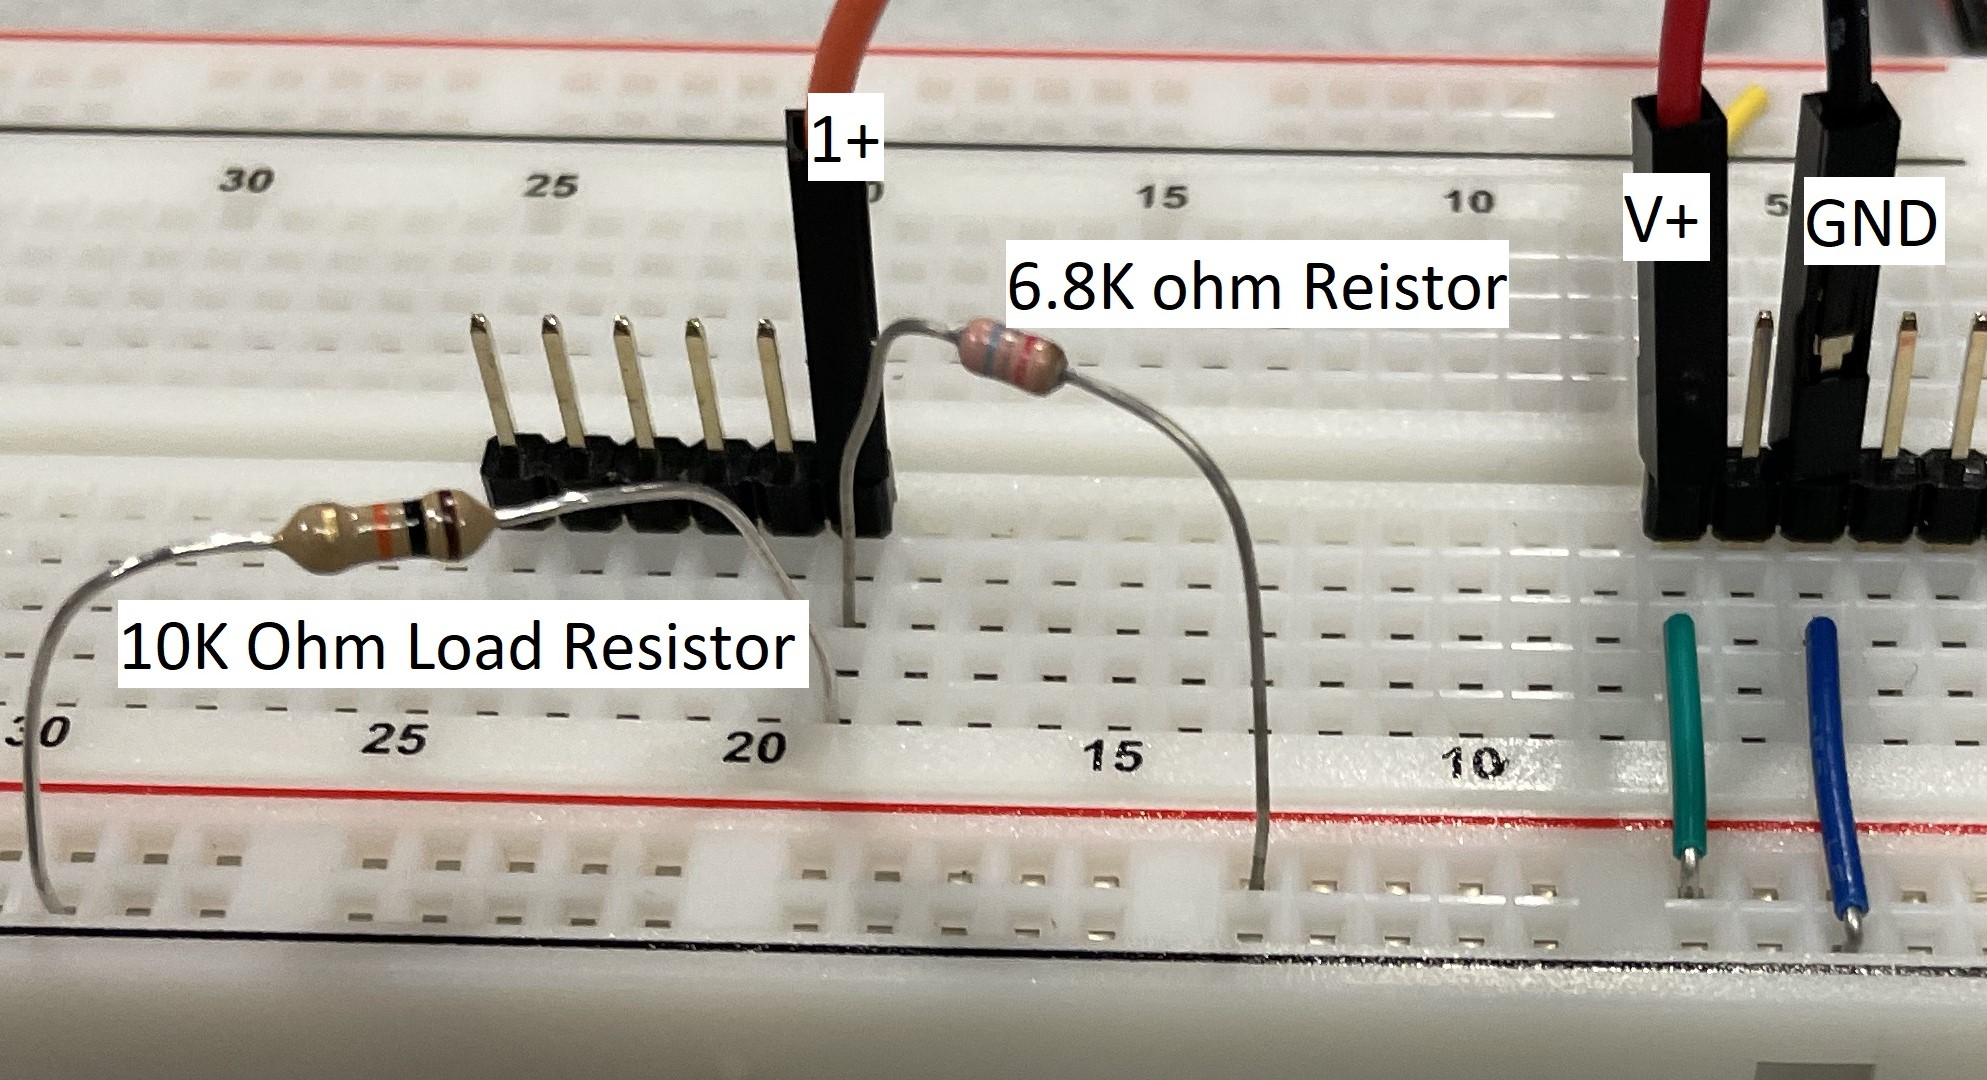
\includegraphics[width=8cm]{Lab2 Equivalent Circuit}
\centering
\caption{Lab 2 Equivalent Circuit}
\end{figure}
\section*{Measurements: Lab 2}
\begin{center}
\begin{tabular}{|c|c|c|c|c|c|}
\hline
$V_{th}$ & $I_N$&$R_{th}$&$V_{OC}$&$I_{SC}$&$R_{eq}$\\
\hline
2.966V & 0.452mA & $6.56K\Omega$ & $2.97V$ & 0.432mA & $6.827K\Omega$\\
\hline
\end{tabular}
\end{center}
The equivalent circuit I created was a $6.8\Omega$ resistor in parallel with a $2.97V$ voltage source. The voltage across the load resistor in this case was $1.777V$ compared with $1.79V$ in the actual circuit.
\pagebreak
\section*{Discussion: Lab 2}
For the comparison of the voltages across the load resistors in the actual and equivalent circuit, see the measured voltages above. \\
\\
The power dissipated by the load resistor is
$$P_{R_{L}}=\frac{R_L}{(R_{th}+R_L)^2}V_{th}^2$$
This is maximized when $R_L=R_{th}$.
\pagebreak
\section*{Experiment: Lab 3}
\begin{figure}[h]
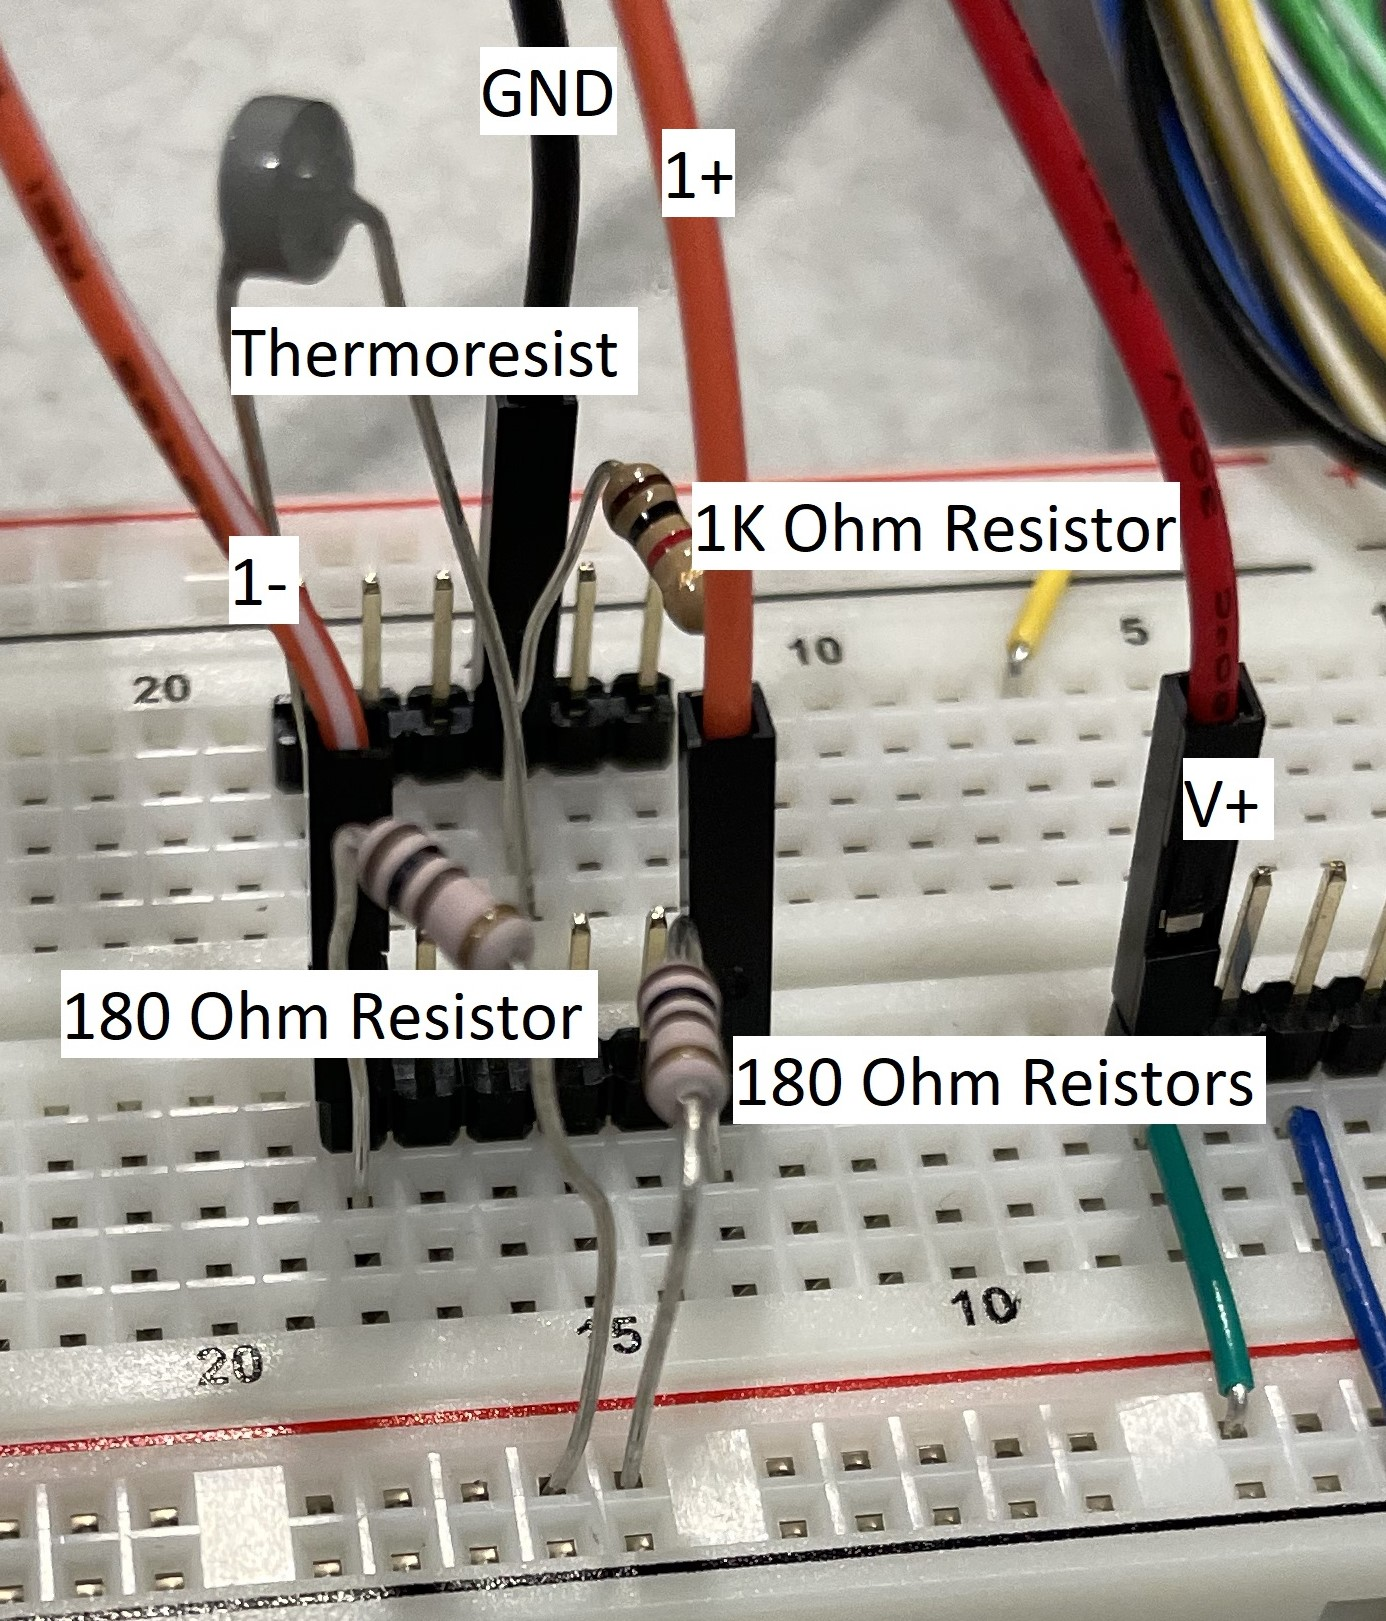
\includegraphics[width=8cm]{Lab3 Circuit}
\centering
\caption{Lab 3 Circuit}
\end{figure}
\section*{Measurements: Lab 3}
Room Temperature
$$V=2mV$$
Body Temperature
$$V=0.232mV$$
\pagebreak
\section*{Discussion: Lab 3}
The temperature sensor is not biased away from 0, furthermore this circuit was not as susceptible to voltage changes, a change of $1V$ in the input voltage would only result in a $0.04V$ change in $V$.
\pagebreak
\section*{Conclusion}
In this lab we understood how to apply Thevenin and Norton equivalence theorems. We experimentally verified and measured the principle of superposition. And we understood the operation of the Wheatstone bridge, and how it would apply to constructing circuits with sensors. 


\end{document}